\section{Realization}
\label{sec:realization}
%Focus generale sulle tecnologie utilizzate
In this section, we outline the technical aspects concerning the realization of our approach. Therefore we first present the enabler technologies through which we instantiate the design principles presented in \cref{sec:design}. After that, we discuss the interaction workflow between the instantiated technologies. Finally, we show the implementation details.
\begin{figure}[t]
\centering
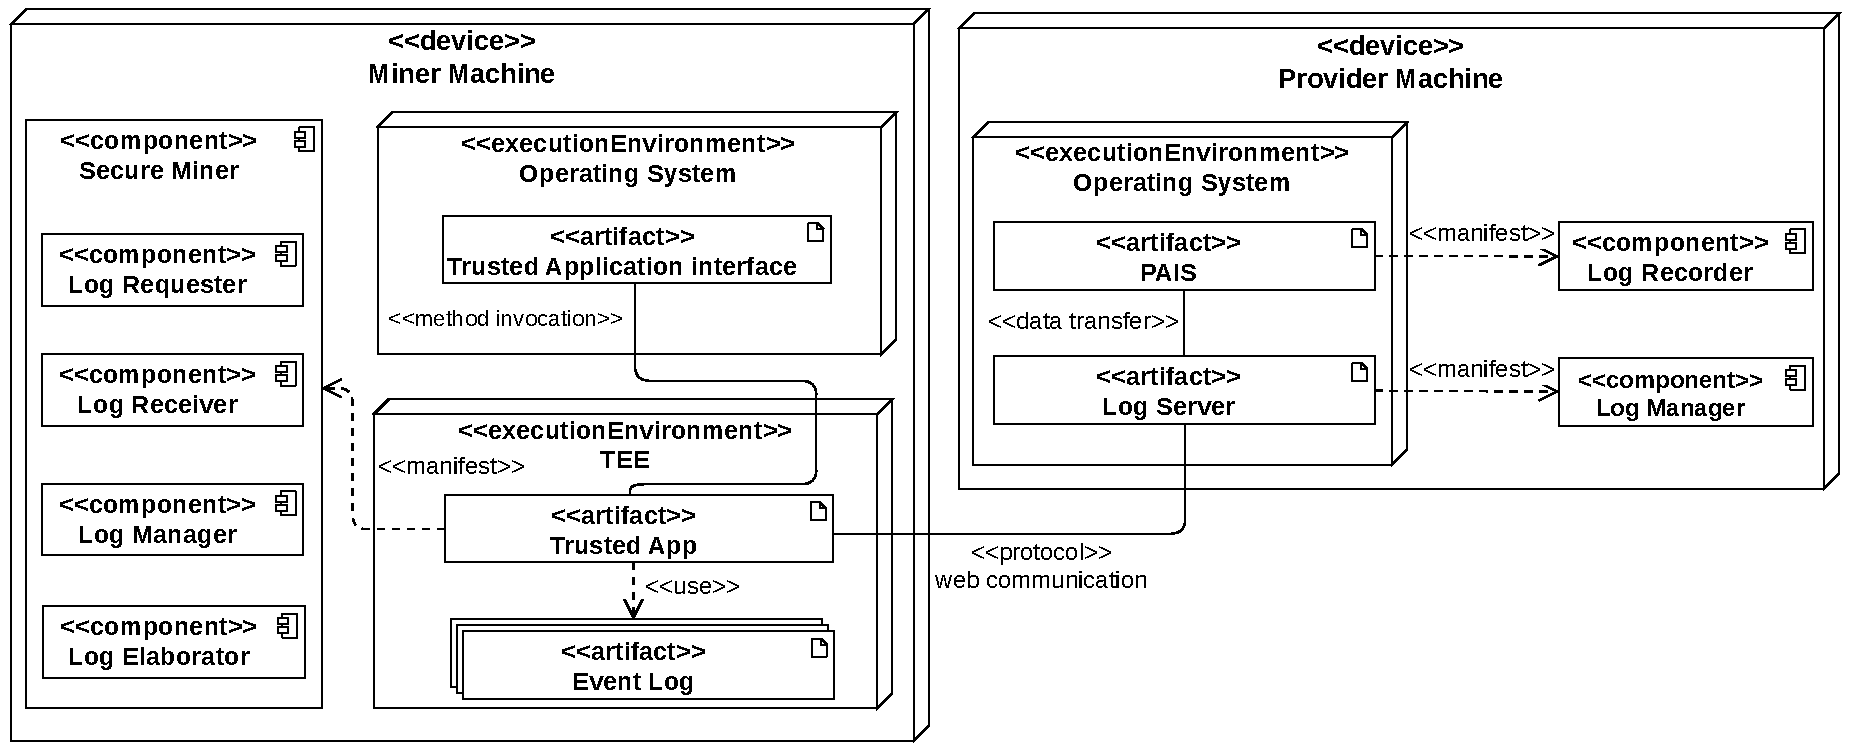
\includegraphics[width=1\linewidth]{content/figures/deploymentdiagram2.pdf}
\caption{UML deployment diagram.}
\label{fig:deployment_diagram}
\end{figure}
\subsection{Deployment}
As follows, we bridge the gap between high-level system architecture and its practical realization. \cref{fig:deployment_diagram} depicts a \textit{UML deployment diagram} \cite{koch2002expressive} that aims to help with understanding the instantiated infrastructure. 

The \texttt{Organization Machine} represents the physical computation \textit{device} embracing the software and hardware entities of the company. The \texttt{Log Recorder}, the \texttt{Log Provider}, and \texttt{Secure Miner} are included in the \texttt{Organization Machine} as abstract \textit{components}. These logical elements incorporate the core functionalities already discussed in \cref{sec:design}. The \texttt{Organization Machine} is characterized by two \textit{execution environment}s, namely the \texttt{Operative System} and the \texttt{TEE}.

Software entities we expose to the users of the \texttt{Organization Machine} run inside the \texttt{Operative System}. We manifest the functionalities offered by the \texttt{Log Recorder} in the \texttt{PAIS}  \cite{Dumas.etal/2018:FundamentalsofBPM}. These systems help users to handle business processes, including accounting and resource management. In our solution, the \texttt{PAIS} provides the \texttt{Log Server} access to event logs. \texttt{Log Servers} are web services that process remote data request and provides event log to miners. We build these entities upon existing web standards such as HTTP\footnote{\url{https://www.w3.org/Protocols/rfc2616/rfc2616.html}. Accessed: \today.}, FTP\footnote{\url{https://www.w3.org/Protocols/rfc959/}. Accessed: \today.}, and Goopher\footnote{\url{https://datatracker.ietf.org/doc/html/rfc1436}. Accessed: \today.}.

\texttt{TEE}s create a separated context from the normal \texttt{Operating System} to protect code and data through hardware-based security features in a reserved zone of the \texttt{Organization Machine}'s CPU. We leverage the security guarantees offered by these technologies to instantiate a \texttt{Trusted Application} to fulfill the functionalities of the \texttt{Secure Miner} and its subcomponents. The \texttt{Trusted Application} collects the logic to generate verifiable data requests, receive external event logs, store them in the \texttt{TEE}, and apply process mining algorithms. Procedures executed by the \texttt{Trusted Application} are tamperproof. The \texttt{TEE} ensures that the code of the \texttt{Trusted Application} executed within it is protected from unauthorized access and malicious manipulations. We employ the isolated context of \texttt{TEE} to store \texttt{Event Log}s of partner organizations inside the miner machine. The \texttt{TEE} provides a mechanism to protect this sensitive information without exposing it to the \texttt{Operative System}. The \texttt{Trusted Application} is the only entity that can access the \texttt{Event Log}s and feed them to process mining algorithms. Users can communicate with the \texttt{Trusted Application} via the \texttt{Trusted Application Interface}. The \texttt{Trusted Application} offers secure methods to safely receive information from the \texttt{Operative System} and present the outputs of the computation. These methods are invoked by the \texttt{Trusted Application Interface} and instantiate the only communication channel to the \texttt{Trusted Application}.
\begin{comment}
\begin{figure}[t]
\centering
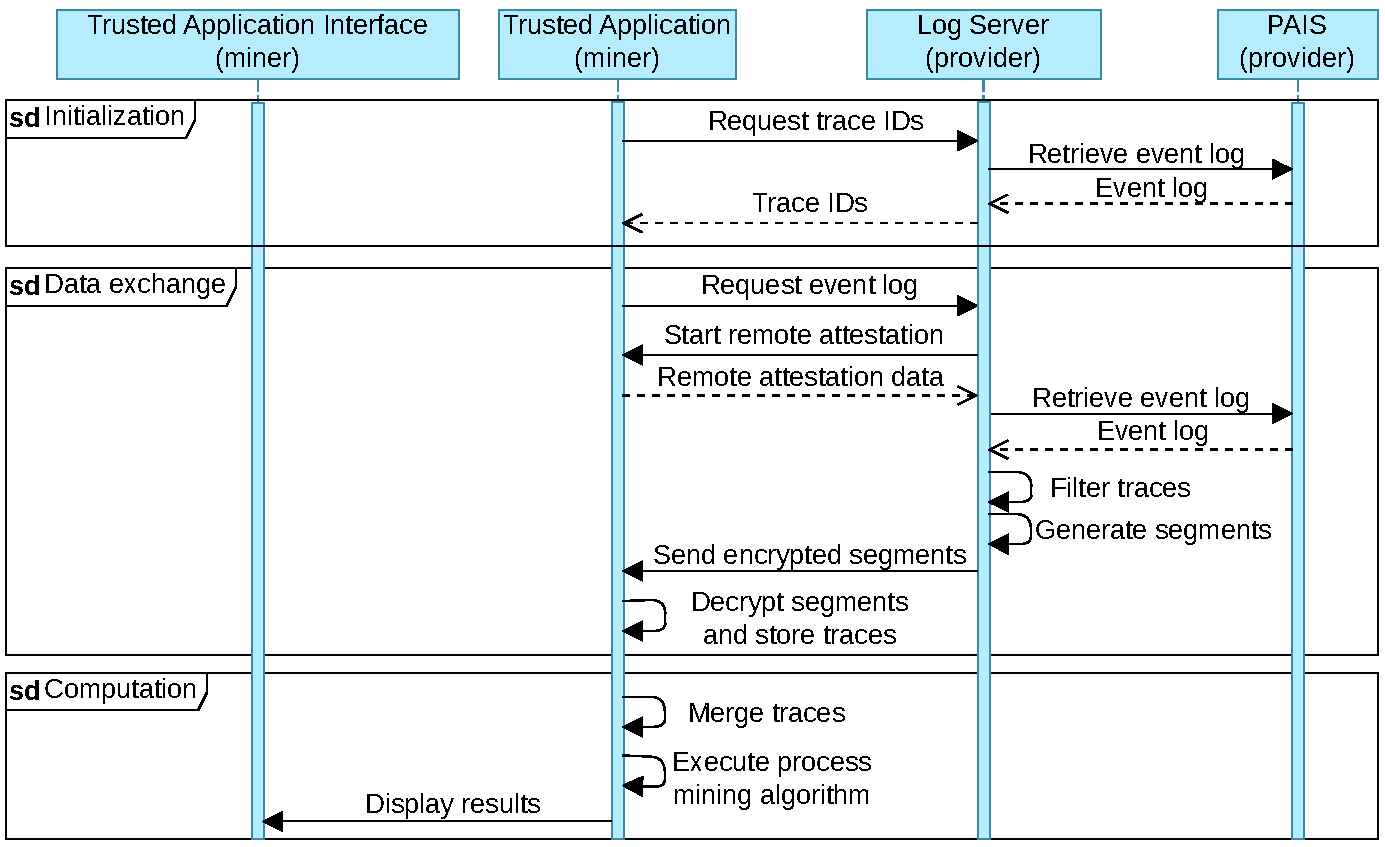
\includegraphics[width=0.9\linewidth]{content/figures/sequencediagram.pdf}
\caption{UML sequence diagram.}
\label{fig:sequence_diagram}
\end{figure}
\end{comment}
% \begin{comment}
    \begin{figure}[t]
     \subfloat[][Initialization]{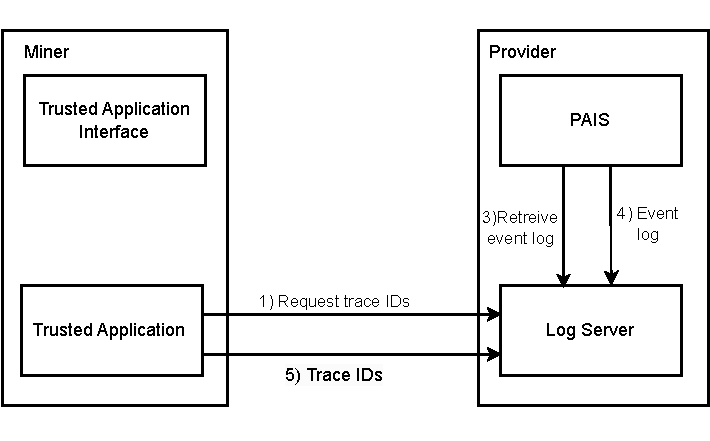
\includegraphics[width=0.3\linewidth]{content/figures/flow_Initialization.pdf}\label{<figure1>}}
     \hfill
     \subfloat[][Remote Attestation]{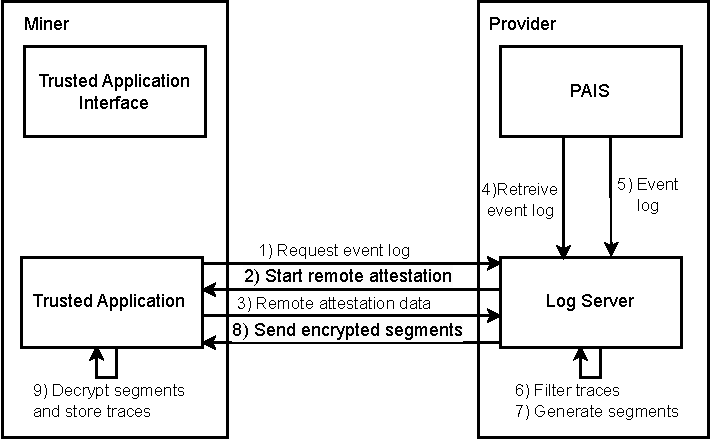
\includegraphics[width=0.3\linewidth]{content/figures/flow_dataExchange.pdf}\label{<figure1>}} 
     
     \subfloat[][Data Exchange]{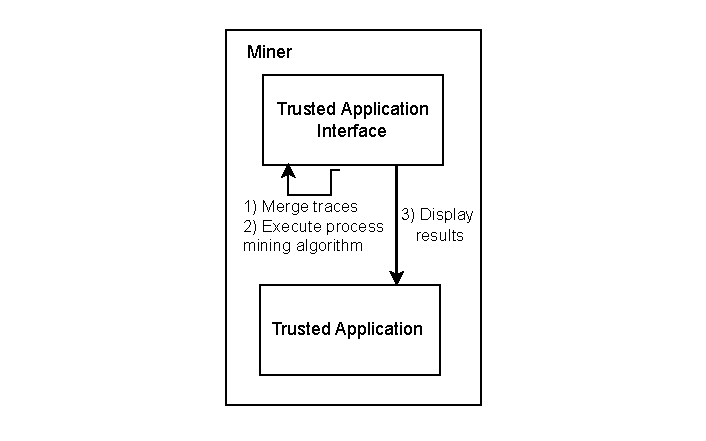
\includegraphics[width=0.3\linewidth]{content/figures/flow_computation.pdf}\label{<figure1>}}
     \hfill
     \subfloat[][Computation]{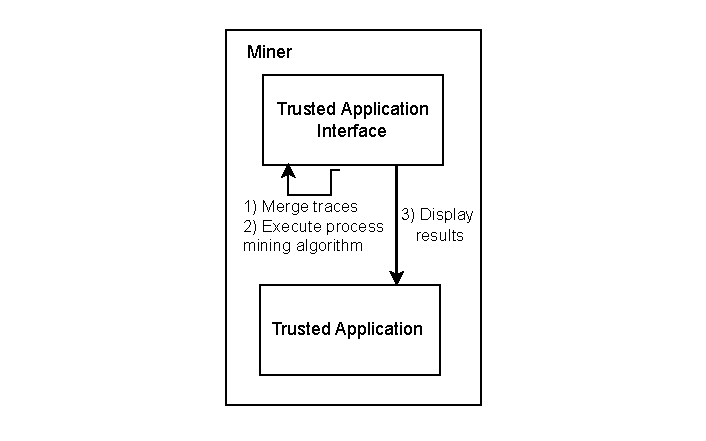
\includegraphics[width=0.3\linewidth]{content/figures/flow_computation.pdf}\label{<figure1>}}
     \label{flow}
\end{figure}
% \end{comment}


\subsection{Interaction flow}
As follows, we analyze the data flows and interactions among the introduced technologies. We separate the workflow into subsequent processes, namely \textit{initialization}, \textit{data exchange}, and \textit{computation}.
The parties involved in the workflow are a miner (i.e., an organization that executes process mining algorithms) and one or more providers (i.e., partner organizations that serve their event logs). %We distinguish three different phases of the process namely the \textit{initialization}, the \textit{data exchange}, and the \textit{computation}.
\todo{CDC: We need an example. We must provide an example of (simplified) event log excerpt, with a few traces taken from the scenario, show which bits reside in the different machines, and show the final merged event log. Then, discuss it during the description of the workflow, showing how we get from the original pieces to the final one. This description takes time.}

\textbf{Initialization.} In the initialization, the miner's \texttt{Trusted Application} requests preliminary information from the providers' \texttt{Log Server} concerning the event logs of an inter-organizational business process. After authenticating the sender, the involved \texttt{Log Server}s retrieve the local event log from the \texttt{PAIS} and respond to the miner by providing the list of trace IDs in the event log. Hence, the \texttt{Trusted Application} collects the responses and stores them in the \texttt{TEE}.
\textbf{Remote Attestation.} \todo[inline]{Talk specifically of remote attestation}
\textbf{Data exchange.} Once recorded the preliminary information, the miner starts the data exchange. Therefore, its \texttt{Trusted Application} sends data requests to the \texttt{Log Servers}. The requests include as parameters the list of trace ids and the segment size. Subsequently, the \texttt{Log Server}s starts the \textit{remote attestation} procedure, thanks to which they can verify that the sender of the log request: is a \texttt{Trusted Application} running inside a \texttt{TEE}; comes from a partner organization. This operation involves the exchange of additional messages between the \texttt{Log Server} and the \texttt{Trusted Application}. If the procedure is successful, the miner's identity is verified.
Subsequently, the \texttt{Log Servers} retrieve the local event log and filter its traces according to the trace IDs sent by the \texttt{Trusted Application}. Filtered event logs are split into several segments containing traces whose dimension does not exceed the segment size parameter. \texttt{Log Servers} encrypts the segments and send each of them to the \texttt{Trusted Application}. The \texttt{Trusted Application} decrypts the received segments, extracts the traces, and stores them in \texttt{Event Log}s inside the \texttt{TEE}.

\textbf{Computation.} To start a computation routine, the \texttt{Trusted Application} needs all partner organizations to have delivered traces having the same ID. When this occurs, the \texttt{Trusted Application} merges external traces with the owned one. Assembled traces are used as parameters of process mining algorithms executed by the \texttt{Trusted Application} that presents the computation results to the users via the \texttt{Trusted Application Interface}.







\subsection{Implementation}
\label{sec:implementation:details}
\todo[inline]{It can be reduced}

In this section, we describe the implementation of our paper. The implementation proposed integrates a trusted application running in a
trusted execution environment and some event logs generated to address the solution proposed in the motivating scenario. The code is available at the following address: \url{https://github.com/dave0909/TEExProcessMining/}

We have encoded a well-known process discovery algorithm within the \texttt{Secure Miner} component to demonstrate the capability of conducting process analytics tasks with our approach.
\todo{Modify and reposition as needed}



\begin{comment}
\todo[inline]{This is part of the evaluation. Move it wherever appropriate in the next section.}
In order to generate the logs for the execution of the trusted application, we produced a simulation model based on our running example (see~\cref{sec:motivating}).% was created based on BPMN notation\footnote{https://www.bpmn.org}. Subsequently, the model was imported fed as input into the BIMP tool.%
\footnote{https://bimp.cs.ut.ee}
% which made it possible to generate the synthetic event logs. 
The number of log traces generated through BIMP aligns with other works in the state of the art; the generation software was set to 1000 traces.
\todo{Mention Sepsis here}
Following the generation, the synthetic event log relating to the process model was filtered via ProM.%
\footnote{https://promtools.org}
We were able to filter the logs based on attribute values, which allowed us to filter the synthetic log according to the resource involved in the activities. Referring to the motivating scenario, the resources involved are the hospital, the specialized clinic, and the pharmaceutical company. In this way, we created three separate event logs from the initial event log, which were used to exchange data between the organizations.
\end{comment}

To implement the trusted applications, we used the EGo,%
\footnote{https://www.edgeless.systems/products/ego/} 
a framework to encode programs for TEEs in %. EGo makes it possible to develop trusted applications programmed in 
GO.%
\footnote{https://go.dev}
% We developed the Trusted Application (TA) within the TEE with the same language. 
Within the TA there is the ``Secure Miner" module, which allows logs from other organizations to be requested, managed, and processed. Log processing is made possible by the implementation of the ``Heuristc Miner" process mining algorithm\ref{weijters2006process}, which takes the log traces as input and performs a discovery operation.
The output of the algorithm is a PNML\footnote{https://www.pnml.org}(Petri Net Markup Language) which allows the representation of Petri nets that graphically illustrate the model calculated by the algorithm. 
%The output of the algorithm is a file with the extension '.pnml'. PNML\footnote{https://www.pnml.org}(Petri Net Markup Language) is a markup language that allows the representation of Petri nets that graphically illustrate the model calculated by the algorithm. 
In order to generate the graphic image of the Petri net, we used the WoPed\footnote{https://woped.dhbw-karlsruhe.de} software, which takes as input a PNML file and provides the graphic representation of the Petri net. 

%Log provider language
Another fundamental module within the TA is the Log Provider. We wrote this part of TA in Go. The log provider is listening for log requests from other organizations on one of the ports set by the owning organization. When an organization decides to start the mining process, it requests the logs of the other organizations. The log providers accepts requests made by the organization that starting the mining operation and forwards its log.